\documentclass[a4paper]{report}

\usepackage{graphicx}
\usepackage{float}
\usepackage[margin=1.0in]{geometry}

\title{Foot Pressure Analyzing Shoe}
\date{2016.14.06}

\begin{document}
	
	\maketitle
	
	\tableofcontents
	
	\newpage
	
	\section{Introduction}
	\paragraph{}
	At the beginning of the civilization, humans used to cover the foot with skin of the animals. Since then shoes have evolved so much. Today they are an important accessory of the day to day life. In the modern world shoes are designed for various purposes. They are not just utilities that provide comfort and protection for feet but a fashion item. 
	Various types of shoes are produced for different tasks. Some shoes enhance the movability, some give protection from harsh environment conditions while others are purely for aesthetic qualities. Demand for task-specific footwear shows an exponential growth today with the marketing trends and increase of population. Designing a shoe is an important task because incorrect design may lead to incorrect posture or gait will ultimately result in conditions such as muscle pain. Therefore it is useful to analyze the pressure distribution of the foot to decide the best design for the footwear.
	
	\paragraph{}
	The field of analyzing the pressure between the foot and the surface is known as Pedobarography. The ways to measure the pressure exerted by foot can be categorized mainly as floor-based and in-shoe systems. The data gathered in these means are extremely important for biomedical and sports applications. As an example, gait analysis of sportsmen can be used to derive new techniques which can enhance movement speed or reducing the stress. And also analyzing the planter pressure of elderly people may reveal more about the root causes for diseases that are common among the elderly community. Therefore number of shoes have been introduced for measuring different biological functions. Various modules are installed in shoes for specific tasks. There are shoes which can monitor the distance walked, heart rate, calories burned etc. 
	
	\paragraph{}
	From the above two methods, in-shoe method has proved to be more practical than the floor-based systems. The main advantages of in-shoe based pressure measurements are low cost, better usability. Other qualities that should be present in such a design should be accuracy of the measurements over continuous stress for a long duration and not giving any discomfort to the user. The purpose of this research is to develop a new in-shoe based foot planter pressure measuring system, overcoming the disadvantages of the current methods that are being used.
	
	\newpage
	
	\section{Technical specifications}
	
	\paragraph{}
	All the means of measuring foot pressure gives some level of discomfort to the wearer. So the primary focus is to design the shoe so as that, the user cannot distinguish it from a normal shoe.
	
	\begin{enumerate}
		\item
		 Fifteen FSR 400 pressure sensors are used inside the sole for gait analysis \ref{fig:sensor_grooves}. Due to the relative less thickness of the sensors, the thickness of the sole is almost indistinguishable from that of a regular shoe. These sensors are manufactures by a third party and are being used widely for pressure measurement due to their small thickness and reliability over a long period.
		 
		 \begin{figure}[H]
		 	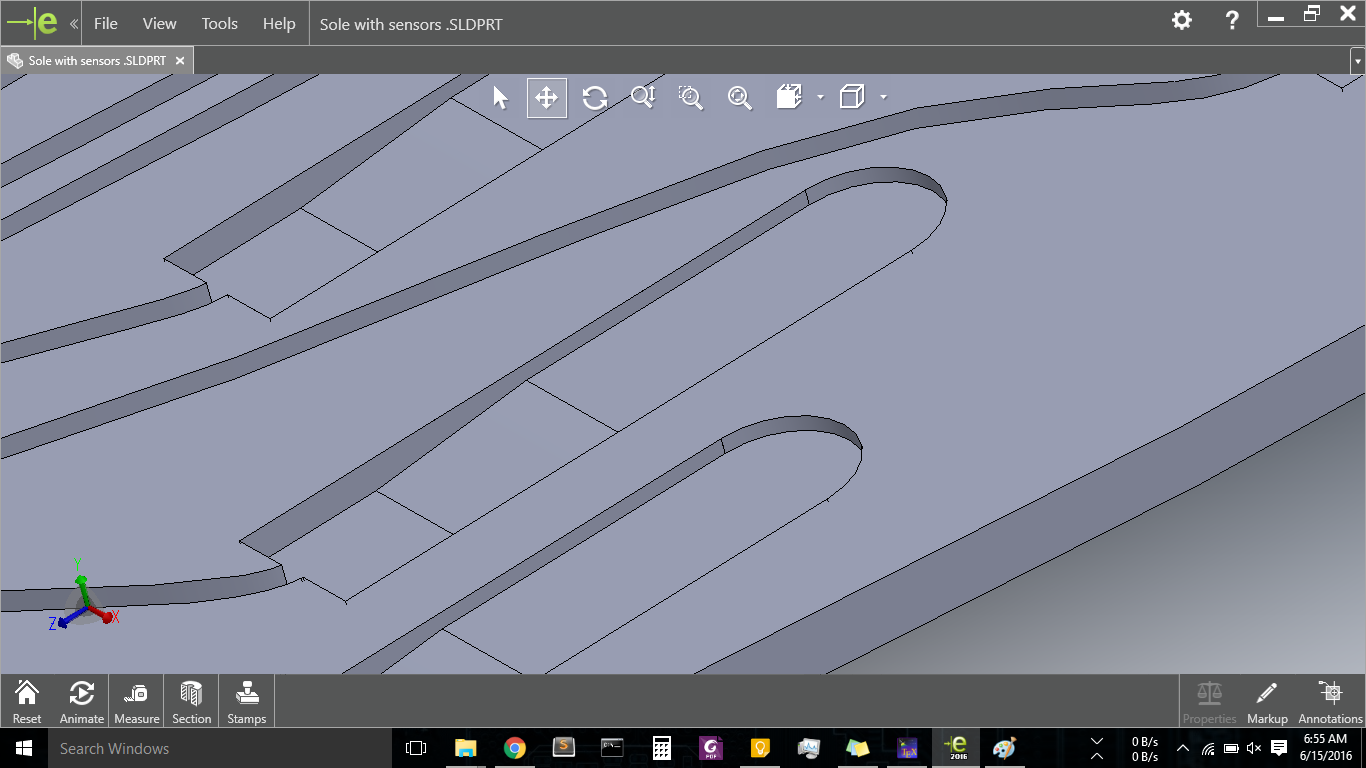
\includegraphics[width = \linewidth]{sensor_grooves}
		 	\caption{Placement of sensors inside the sole}
		 	\label{fig:sensor_grooves}
		 \end{figure}
		
		\item
		The shoe is only expected to work as a transceiver module which transmit the sensor data. The idea is to preserve battery life as much as possible by not processing the data within the shoe.
		
		\item
		Transmitted data being received by the mobile phone of the user is a practical approach for a user who is using the shoe in a non-testing environment. A significantly low energy consumption is expected to achieve by using Bluetooth 4.0 LE.
		
		\item
		This new design poses few advantages over the current planter pressure measurement systems. Since design does not bring any inconvenience or discomfort to the user, the user can wear the shoe for all the regular activities in the natural state. Thus the device is able to collect data in any environment.
		
		\item
		The device is powered by 400mAh Li-ion battery which will run out of power only after hours of use. Therefore it can be used through the day without any inconvenience and plugged to be charged at the end of the day.
		
		\item
		It does not need any other accessory to collect and process the data other than the user’s mobile phone.
		
		\item
		The shoe can be configured to automatically connect and start sending data when the user switch on the Bluetooth service of the phone. This can significantly increase the usability of the device as it also does not need much effort to maintain the device.
		
	\end{enumerate}
	
	\begin{figure}[H]
		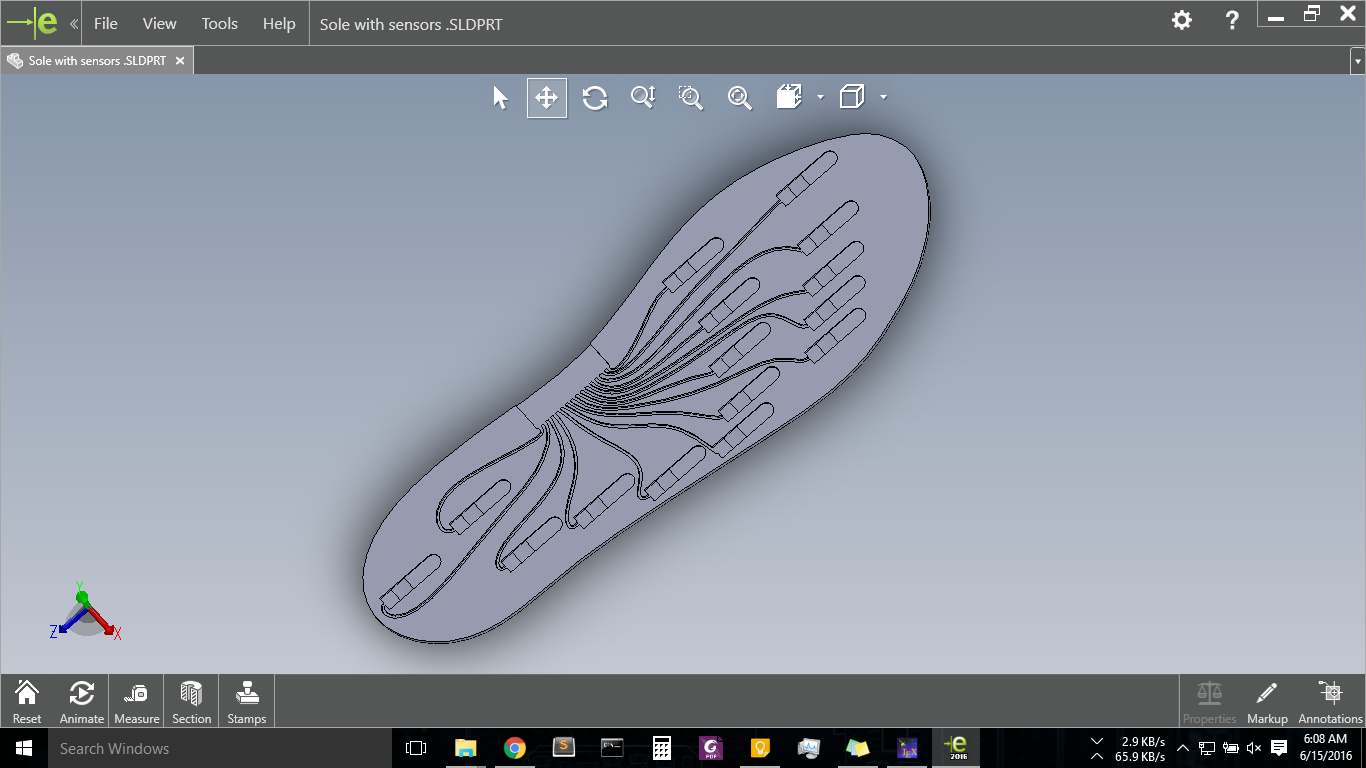
\includegraphics[width = \linewidth]{sole_with_sensors}
		\caption{Sole with sensors}
		\label{fig:sole_with_sensors}
	\end{figure}
	
	\begin{figure}[H]
		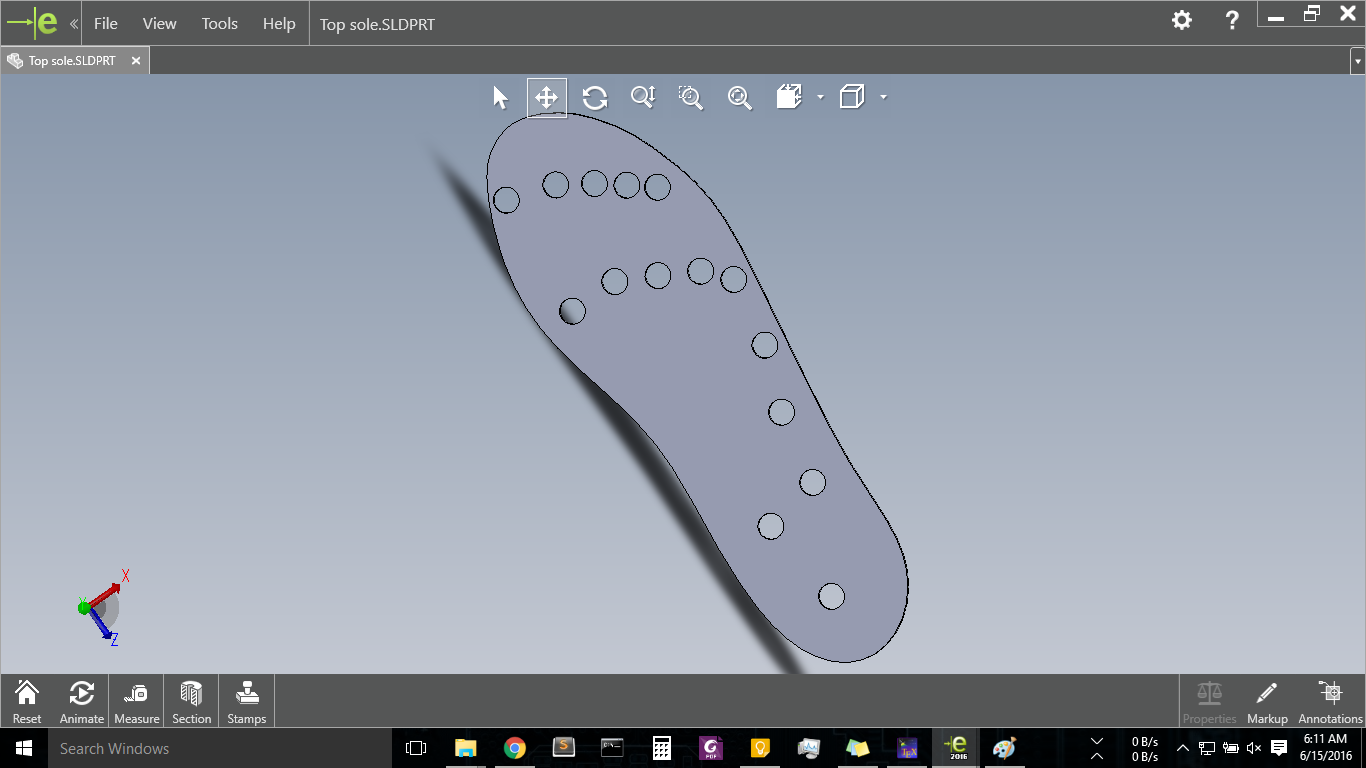
\includegraphics[width = \linewidth]{top_sole}
		\caption{Top sole}
		\label{fig:top_sole}
	\end{figure}
	
	\newpage
	
	\section{Software}
	Software is developed to connect with the shoe and analyze the collected data.
	
	\begin{figure}[H]
		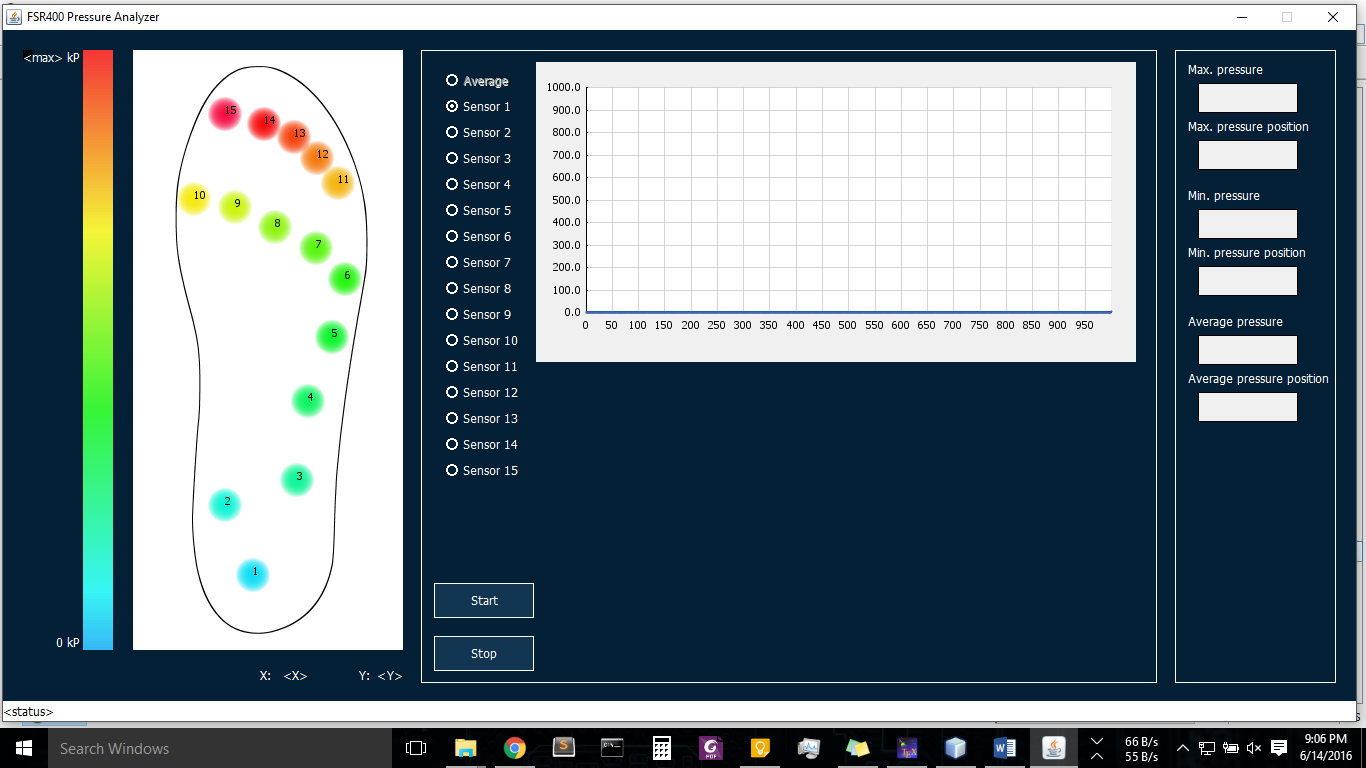
\includegraphics[width = \linewidth]{dashboard}
		\caption{Foot pressure analyzing software - Dashboard}
		\label{fig:dashboard}
	\end{figure}
	
	The input of each pressure point can be analyzed separately or together as an average value. The software can also be configured to receive a live input stream from the shoe. This is more suitable for a development environment.
	
	\newpage
	
	\section{Summary}
	This shoe can be successfully used with the gait analysis of patients and athletes.  By using the collected data, numerous advantages can be gained such as performance improvements of the athletes etc.
	
\end{document}